\chapter{Theoretical concepts and overview of AMBER}\label{cha:theory}
%What is atached in sfh picture
%Mirrored read out has to be explained
%

\section{Measurment of the charge radius of the proton (PRM)}\label{sec:proton_radius}
The proton is a baryon, a composite particle made up of one down quark and  two up quarks.
From this follows that the proton is not a point particle, but has an internal sturucture.
\newline
The internal structure can be discribed by the structure functions of the proton, 
the electric and magnetic form factors $G_E$ and $G_M$. \autocite{ProposalAmber}	
\subsection{Previous measurements of the proton radius}
\begin{figure}[h]
	\centering
	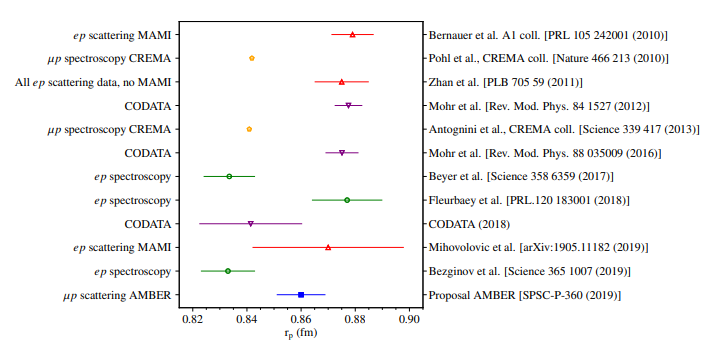
\includegraphics[width=0.8\textwidth]{PreviousmeausrementsProtonradius.png}
	\caption{Previous measurements of the proton radius from electron proton  scattering experiments and the Lamb shift in muonic and ordinary hydrogen,
	 the measurements differ from each other by five standard deviations. \autocite{ProposalAmber} }
	\label{fig:previous_proton_radius}
\end{figure}

The charge radius of the proton has been massured several times before with different methods.
The two premier methods are electron proton scattering experiments and the Lamb shift in muonic and ordinary hydrogen.
The results of these measurements differ by five standard deviations as shown in Figure \ref{fig:previous_proton_radius},
this has given rise to the so called proton radius puzzle. \autocite{ProposalAmber}

\subsection{Elastic scattering of muons on protons}
The AMBER PRM experiment at CERN aims to reslove the proton radius puzzle, by measuring the elastic scattering of muons on protons.
The first order cross section, taking into account only interactions where one virtual photon was exchanged, 
for the elastic scattering of muons on a proton target is 
%INSERT: maybe  here more explantation 
\begin{equation}
\label{eq:cross_section}
\frac{d\sigma}{dQ^2} = \frac{\pi \alpha^2}{Q^4 m_p^2 p_\mu^2} \bigg[ \left( G_E^2 + \tau G_M^2 \right) \frac{ 4E_\mu^2 m_p^2 
- Q^2 (s - m_\mu^2)}{1 + \tau }  - G_M^2 \frac{ 2m_\mu^2 Q^2 - Q^4}{2} \bigg]
\end{equation}
with  $Q^2 = -q^2$ 	the squared transferred four-momentum, $\tau = Q^2 / 4m_p^2$, $s = (p_\mu + p_p)^2$, 
 $G_E$ the electric form factor of the proton,
  $G_M$ the magnetic form factor of the proton and $\alpha$ the fine structure constant. \autocite{intentAmber}
  
  %INSERT: maybe  here more explantation 
Through determining the form factor $G_E$ for small $Q^2$ , the charge radius of the Proton can be claculated with the following equation \autocite{intentAmber}
\begin{equation}
\label{eq:charge_radius}
r_p^2 = -6 \frac{dG_E}{dQ^2} \bigg|_{Q^2 = 0}
\end{equation}

\section{General setup for PRM at AMBER.}\label{sec:general_setup}
\subsection{Detectors for PRM}

To determine the magentic $G_M$ and electric form $G_E$ factors of the proton and thus the charge radius of the Proton,
 the experimental cross section of the elastic scattering of muons on protons has to be measured.

The general setup of the PRM experiment, with focus on the new detectors needed for the proton radius measurment, is shown in Figure \ref{fig:amber_setup}.
\begin{figure}[H]
	\centering
	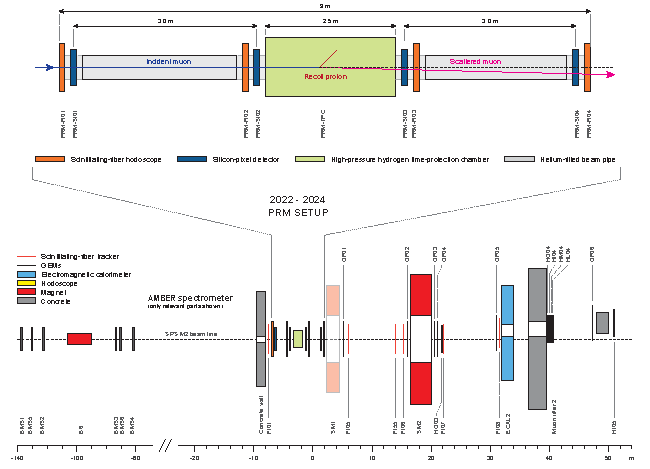
\includegraphics[angle=-90,origin=c,width=0.9\textwidth]{NEWPRMsetup.pdf}
	\caption{General setup of the Amber experiment with new detectors for PRM.
	%INSERT:BETTER DISCRIPTION
	\autocite{InternalcommunicationKarl}}
	\label{fig:amber_setup}
\end{figure}
%INSERT: MAYBE FLUX;ENERGY Maybe include detetor specs 

The incoming muon beam with an energy of \SI{100} {\giga\electronvolt}\autocite{ProposalAmber} and an beam rate of $2 \times 10^6$\autocite{ConfrancePaperDAQ} particles per second is scattered on a pressurized hydrogen gas target, located in the Time Projection Chamber (TPC), 
which also acts as the detector for the recoil path of the scattered proton.
%INSERT: should i included precicion values and other characteristics of the detectors
\newline
The reconstruction of the path of the muon is achieved through the usage of two detector types,
 combined into one unified tracking station (UTS) as shown in Figure \ref{UTSpicture}.
\newline
Each UTS consists of three layers of pixilized silicon detectors (ALPIDEs), for precises positional measurments (spacial resolution of about 8 µm \autocite{Amber2022Status}) of the incoming and scattered muons, 
but lacking the time resolution(\SI{5} {\micro\second}\autocite{Amber2022Status}) required for the PRM experiment.
For this reason each UTS includes a scintillating fiber hodoscope (SFH), the detector of intrest for this thesis,
 which provides the time precision(\SI{300} {\pico\second}\Autocite{Amber2022Status}) for the measurment.
 \newline
Four of these unified tracking stations, two before and two after the active target, are placed in the beamline as shown in \ref{fig:amber_setup}.
The measurment of the momentum of the scattered moun is done by existing COMPASS detectors located after the, 
for the PRM newly included, detectors\autocite{ProposalAmber}.

\begin{figure}[H]	
	\centering
	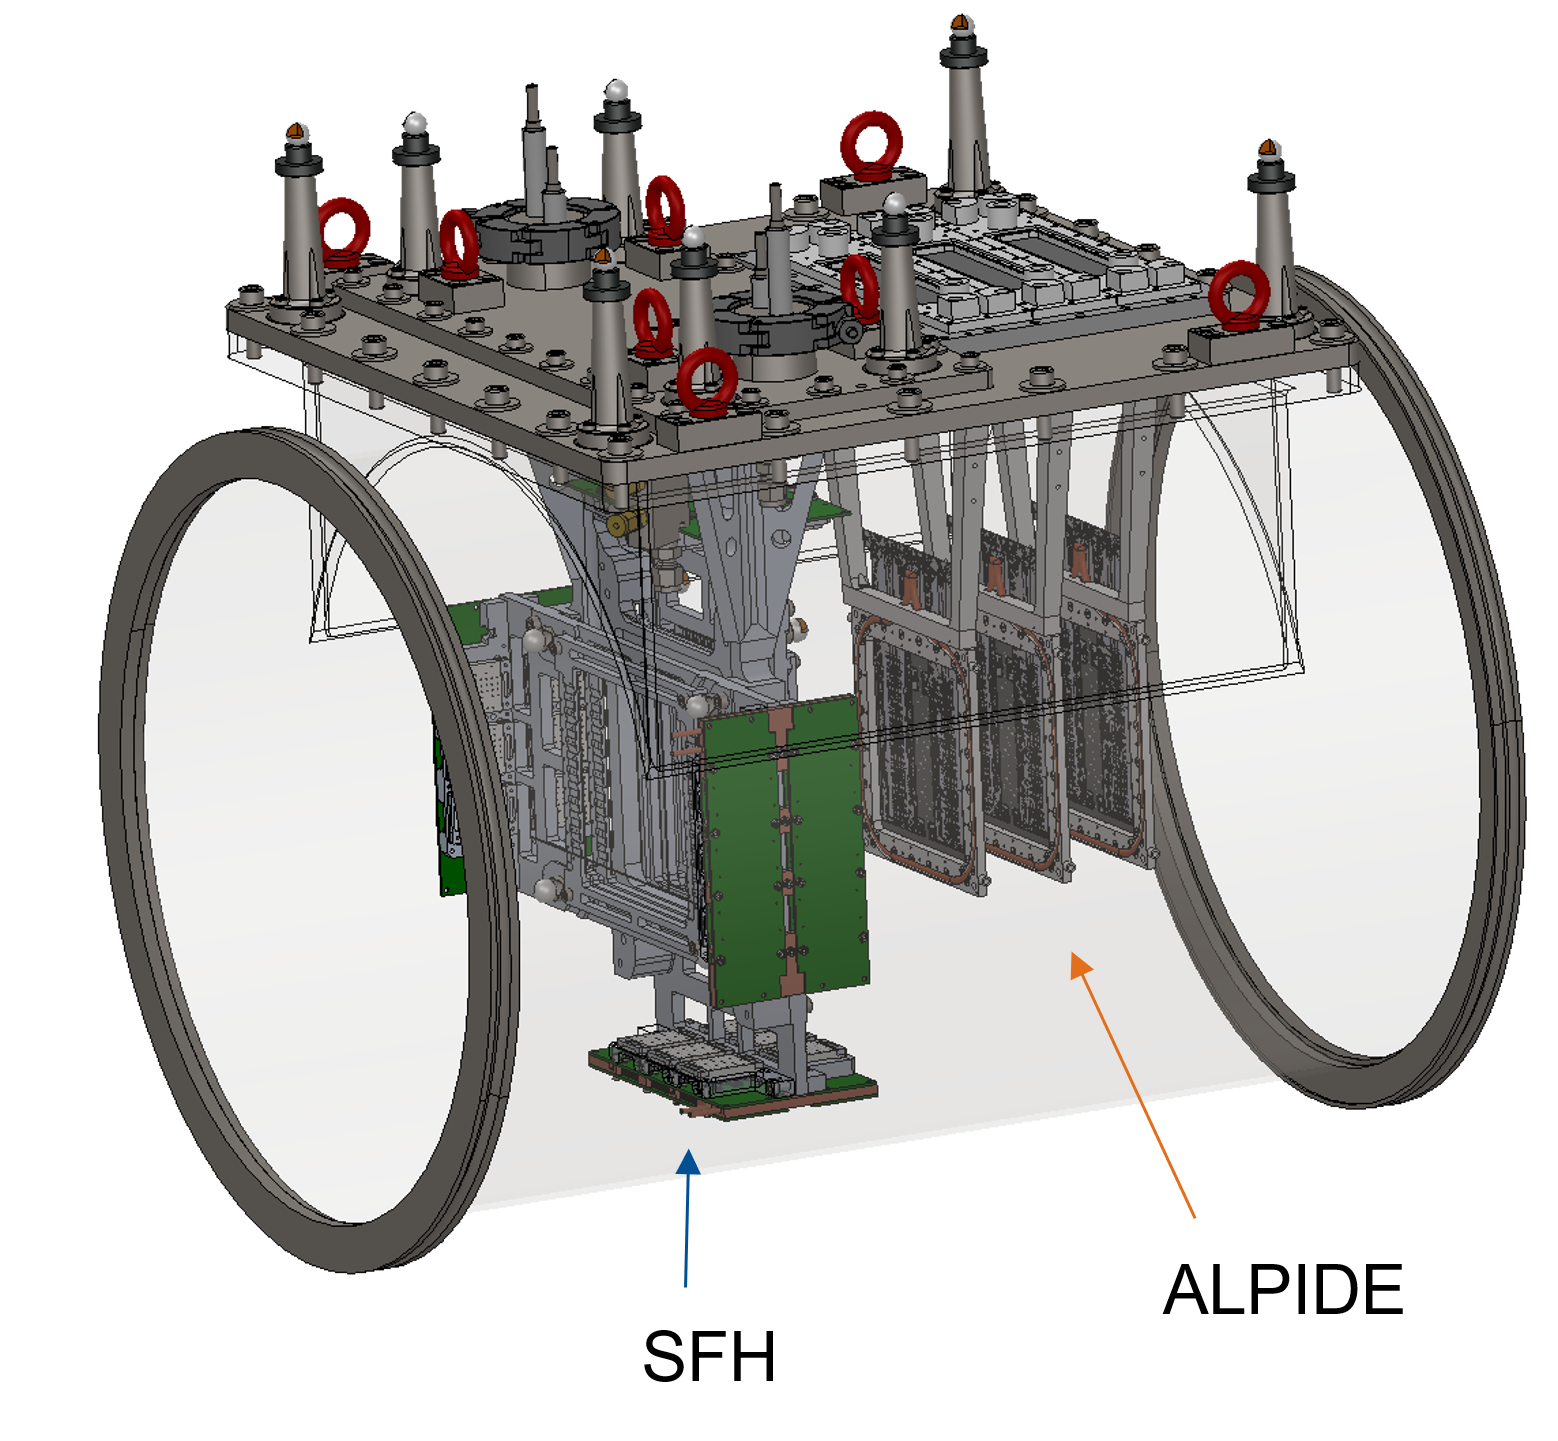
\includegraphics[width=0.8\textwidth]{UFTmodel.png}
	\caption{Unified tracking station (UTS) with three layers of pixilized silicon detectors (ALPIDEs) and the scintillating fiber hodoscope (SFH). \autocite{InternalcommunicationKarl}}
	\label{UTSpicture}
\end{figure}
\subsection{Scintillating fiber hodoscope(SFH)}
\begin{figure}[H]
	\centering
	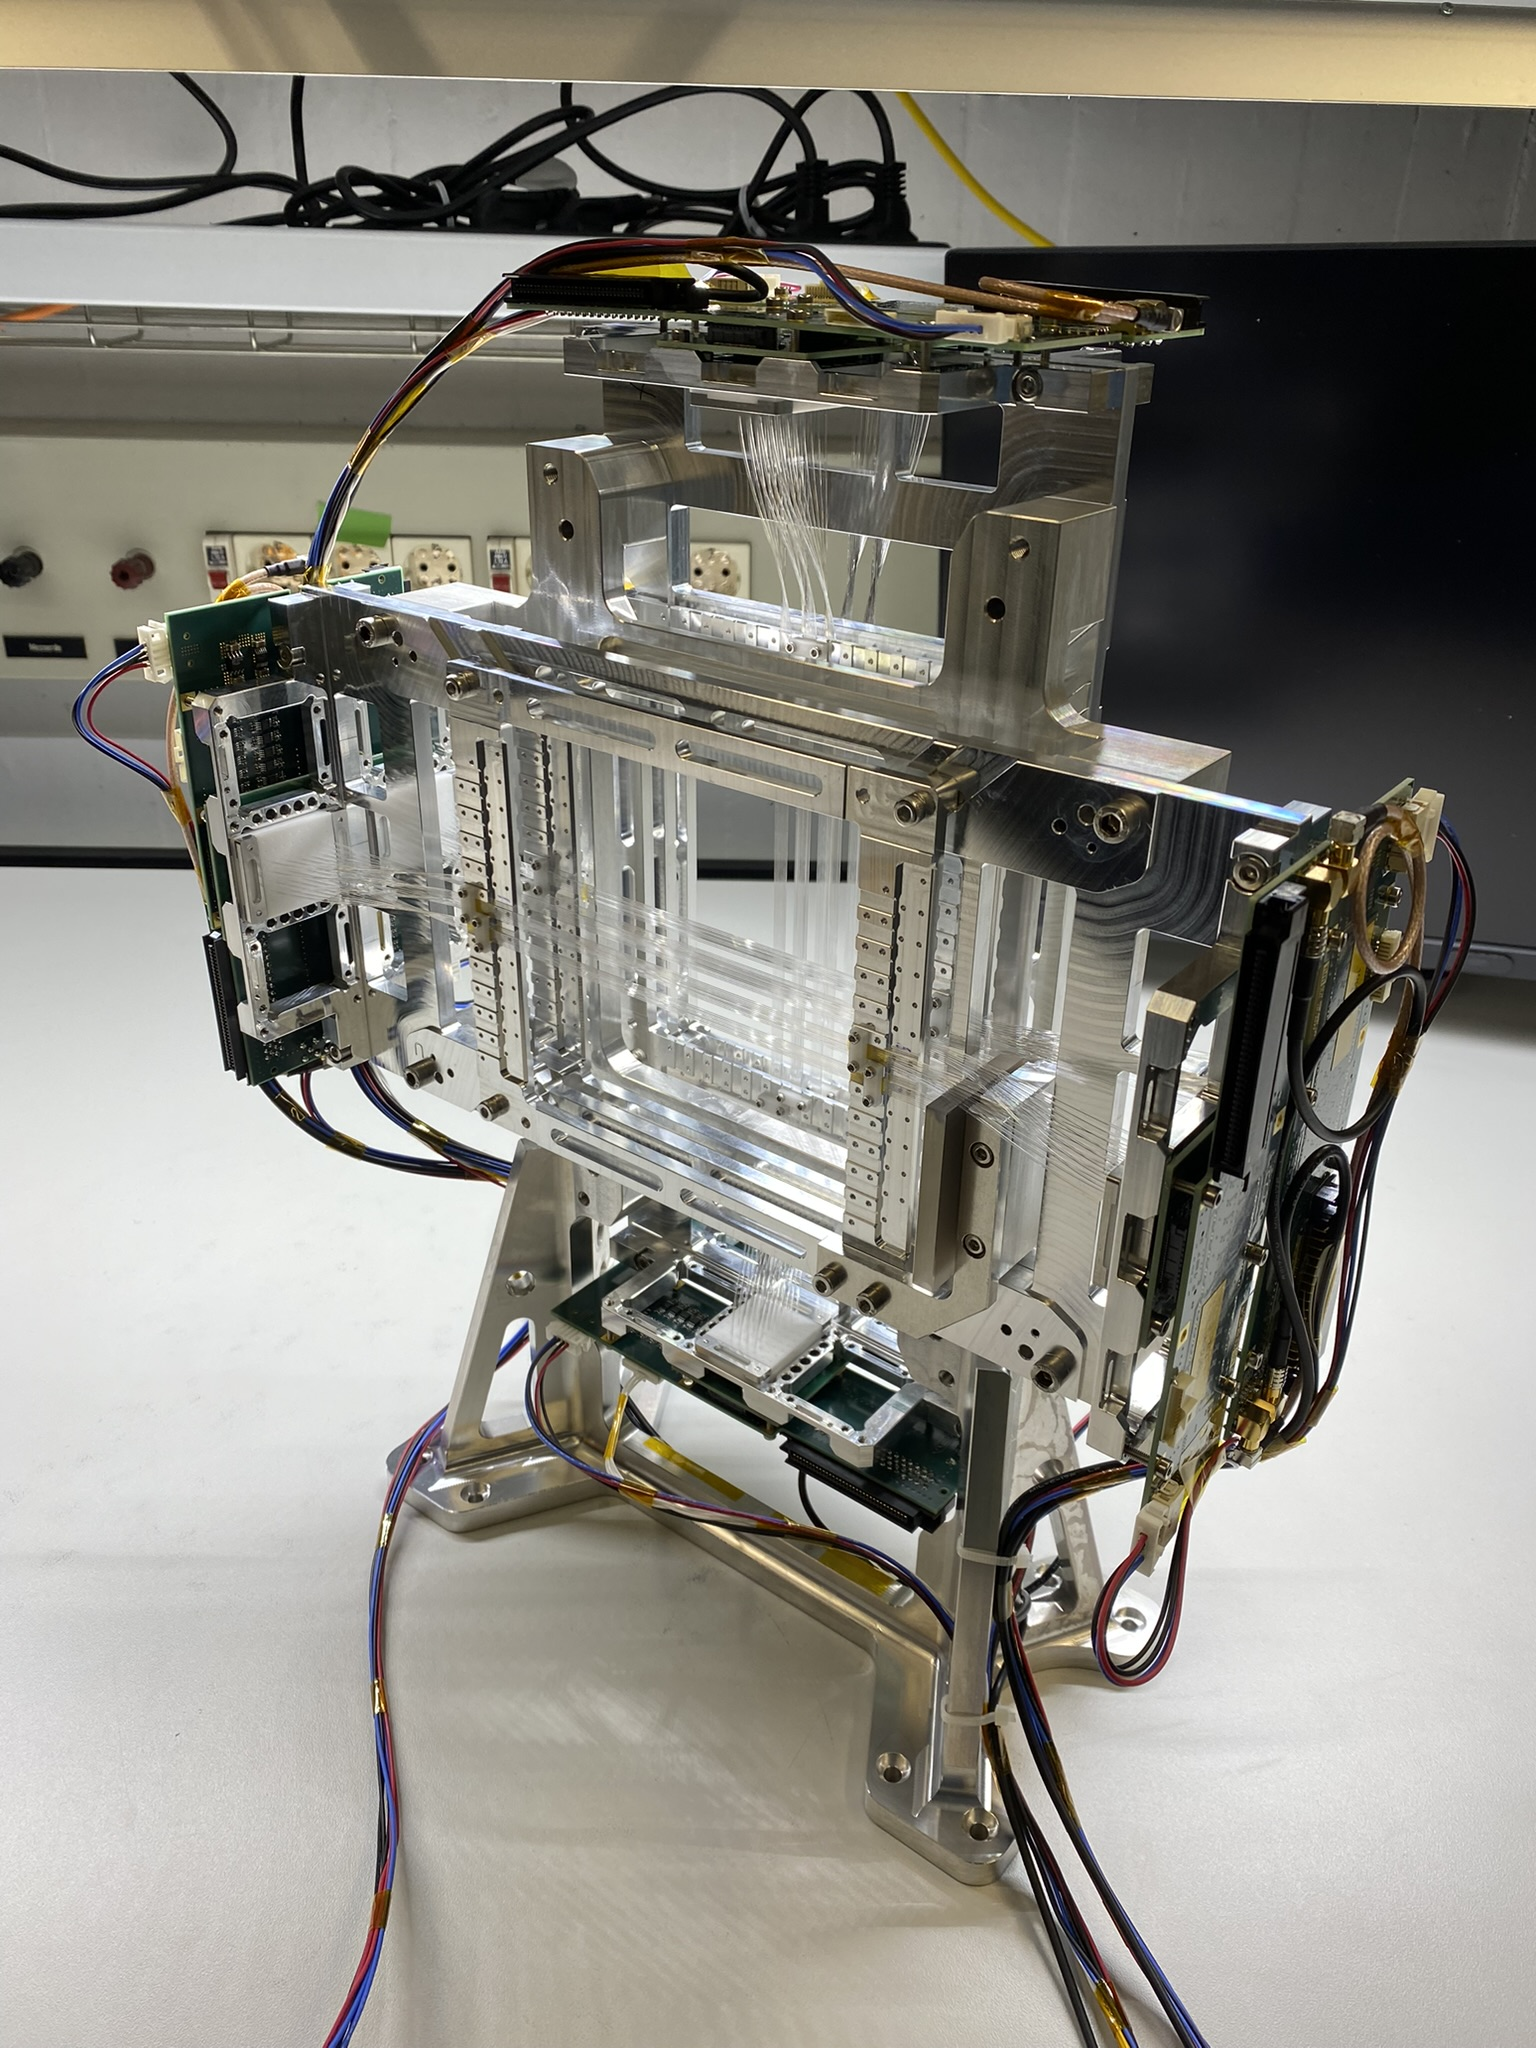
\includegraphics[width=0.8\textwidth]{SFH_somelayers.JPEG}
	\caption{Scintillating fiber hodoscope (SFH) with some of the scintillating fibers of the four layres installed.The frontend electronics are not attached.\autocite{InternalcommunicationKarl}}
	\label{SFHpicture}
\end{figure}
The scintillating fiber hodoscope shown in Figure \ref{SFHpicture}, 
the detector for which the FPGA driven frontend electronics are developed in this thesis,
is used to measure the precise timing(\SI{300}{\pico\second}\Autocite{Amber2022Status}) of the incoming and scattered muons. 
Every SFH contains four layers of scintillating fibers, two in x and two in y direction.
Each layer is made up of 192\autocite{Amber2022Status}, 500 $\mu m$ thick\autocite{Amber2024Status} fibers, in total 768\autocite{Amber2022Status} fibers per SFH. 
When charged particels, muons in this case, pass through a scintillating fiber they excite the scintillating material, 
which then emits photons. Both ends of every fiber are conected to a silicon photomultiplier (SiPM) which converts the photons into an electrical signal,
 that is then proccesed by the frontend electronics. To minimize cost and the amount of data that has to be processed , a mirrored readout is planned, 
 where only one end is conected to the SiPM array and the other end is mirrored. \autocite{InternalcommunicationKarl}

\section{Field Programmable Gate Arrays (FPGAs)}\label{sec:FPGA}
hallo 
